% \documentclass[lineno,twocolumn,endfloat,biblatex]{biophys-new}
\documentclass{biophys-new}
\usepackage[utf8]{inputenc}
\usepackage{graphicx}
\usepackage[colorlinks,allcolors=cyan!70!black]{hyperref}

% uncomment if using biblatex
% \addbibresource{sample.bib}

\usepackage{lipsum}
\usepackage[normalem]{ulem}

\title{Understanding the Free Energy Landscape of Phase Separation in Lipid Bilayer using Weighted Ensemble Molecular Dynamics}
\runningtitle{All plots with long captions} %% For page header

\author[1]{Ashlin Poruthoor}
\author[1,*]{Alan Grossfield}
\runningauthor{Poruthoor and Grossfield} %% For page header

\affil[1]{University of Rochester Medical Center, Rochester, NY 14620}

\corrauthor[*]{alan\_grossfield@urmc.rochester.edu}

% \papertype{Letters}
\papertype{Article}
% \papertype{Computational Tools}


\begin{document}

\begin{frontmatter}
\begin{abstract}

Lorem ipsum dolor sit amet, consectetur adipiscing elit, sed do eiusmod tempor incididunt ut labore et dolore magna aliqua. Ut enim ad minim veniam, quis nostrud exercitation ullamco laboris nisi ut aliquip ex ea commodo consequat. Duis aute irure dolor in reprehenderit in voluptate velit esse cillum dolore eu fugiat nulla pariatur. Excepteur sint occaecat cupidatat non proident, sunt in culpa qui officia deserunt mollit anim id est laborum.

\end{abstract}

\begin{sigstatement}

Lorem ipsum dolor sit amet, consectetur adipiscing elit, sed do eiusmod tempor incididunt ut labore et dolore magna aliqua. Ut enim ad minim veniam, quis nostrud exercitation ullamco laboris nisi ut aliquip ex ea commodo consequat. Duis aute irure dolor in reprehenderit in voluptate velit esse cillum dolore eu fugiat nulla pariatur. Excepteur sint occaecat cupidatat non proident, sunt in culpa qui officia deserunt mollit anim id est laborum

\end{sigstatement}

\end{frontmatter}

\section*{Introduction}

* Why phase separation is important?
* Why phase separation in cell membrane is important?
* Molecular dynamics
* Challenges of simulating phase separation using MD
* Ways to work around - CG. Enhanced sampling 
* Choice of WE

Todo list:

Figures: 

1. A figure showing individual MARTINI lipids and their AA chemDraw figure.
    A figure showing the top and side view of each lipid systems

\section*{Methods}

\subsection*{System details}

As shown in Fig 1, we used three different ternary lipid bilayer systems to test the hypothesis:
1. As the primary test system, we chose a lipid bilayer consisting of dipalmitoyl-phosphatidylcholine (DPPC), dilinoleyl-phosphatidylcholine (DIPC), and Cholesterol (CHOL), known to phase separate in silico in a few microseconds \cite{Risselada2008, Schafer2010, Janosi2012, Doma2012, Jong2013, Liu2020, Su2020}.
2. As a positive control, we chose a lipid bilayer consisting of DPPC, diarachidonoyl-phosphatidylcholine (DAPC), and CHOL, known to phase separate relatively faster in silico in the order of a few hundred nanoseconds \cite{Lin2016, Lin2019, Davis2013a}.
3. As a negative control, we chose a lipid bilayer consisting of DPPC, palmitoyl-oleoyl-phosphatidylcholine (POPC), and CHOL that was previously shown not to phase separate \cite{Veatch2003,Davis2013a}.
The composition of DPPC-DIPC-CHOL, DPPC-DAPC-CHOL, and DPPC-POPC-CHOL systems used here are (0.42/0.28/0.3), (0.5/0.3/0.2) and (0.4/0.4/0.2) respectively and are adapted from previous studies \cite{Risselada2008, Lin2016, Davis2013a}.

Due to the relatively larger system size and time scale required for phase separation and related dynamics in lipid bilayer simulations, we used the Coarse-Grained (CG) model for each system. Hence the subsequent dynamics propagation using MD is relatively cheaper than an All-Atom model but with a tradeoff in system resolution.
The rationale behind this design choice is to fail faster with minimum resources if this proof-of-concept protocol is not working as expected. 
Using CHARMM-GUI Martini Maker \cite{Qi2015}, we constructed four random replicas of each CG ternary symmetric bilayer system.
We used MARTINI 2 force field parameters and particle definitions\cite{Marrink2007, DeJong2013} to construct CG systems and to run the subsequent MD simulation.
We replaced the default input files from CHARMM-GUI Martini Maker with their respective most recent Martini 2.x versions if they existed.
We used MARTINI polarizable water model\cite{Yesylevskyy2010} to solvate all systems with approximately a 1:30 lipid to real water ratio.
A detailed description of the systems is given in Table S1 of supplementary material.

\subsection*{Standard MD simulation details}

Due to the historical compatibility of the GROMACS MD engine with the MARTINI force field, we used GROMACS 2020.3\cite{Abraham2015} to propagate the dynamics of the systems prepared. 
Each system was minimized and equilibrated in steps using the MD input files suggested by CHARMM-GUI Martini Maker.
To obtain an intact bilayer without any membrane undulations, we used an additional membrane restraining protocol: 
We took advantage of the flat bottom restrain potential available in GROMACS to allow lipids to move freely in the $xy$ plane but restrained within a slab of defined z thickness.
More details about membrane restraining protocol are given in the supplementary material.

After the minimization and equilibration, all systems were run at 400 K in the NPT ensemble for 100 ns to make sure the lipids in each system were randomly distributed.
For every system, we forked each replica into multiple temperature runs simulated at different temperatures ranging from 298K to 450K.
All standard MD simulations ran for at least 8 microseconds using the BlueHive supercomputing cluster of the Center for Integrated Research and Computing at the University of Rochester.
Simulations ran on Intel Xeon E5-2695 and Gold 6130 processors augmented with Tesla K20Xm, K80, and V100 GPUs.   
The trajectories were processed and analyzed using the LOOS software package.
A detailed description of the simulation parameters is given in Table S1 of supplementary material. 

\subsection*{Collective Variable}

A collective variable (or a set of variables) is a reduced coordinate that captures the progress of a system along the transition of interest.
Ideally, such a reduced variable(s) should fully capture the key modes of the system to reflect the complex event under study.
The success of any enhanced sampling protocol depends on the chosen collective variable over which the sampling is enhanced\cite{Valsson2016, Yang2019b, Henin2022}. 
Thus to drive the WE simulation, we used three candidates for the collective variable.

\subsubsection*{1. Fraction of Lipids in Cluster (FLC)}
Since the formation of lipid domains with distinct properties from the rest of the bilayer is a characteristic feature of a phase-separating lipid bilayer,
we hypothesized that we could use a variable that quantifies the recruitment of lipids into such domains to track the phase separation events in our systems.
Here, we define the Fraction of Lipids in Cluster (FLC) as follows:

\begin{equation}
\label{eq:CLT}
\text{FLC} = \sum_{i}^{N} \frac{\text{No. of $X_i$ lipids in lipid $X_i$ Clusters}}{\text{No. of Lipid $X_i$}} =  \frac{\sum_{i}^{N} \text{No. of Lipid X$_i$ in Lipid X$_i$ Clusters}}{\text{Total No. of Lipids}}
\end{equation}

Where subscript $i$ denotes the individual lipid species in a bilayer consisting of N total lipid species.
As shown in Figure 2, each system under study has $N=3$ lipid species.
FLC increases as the system goes from a mixed state, with a random distribution of lipids, to a separated state.
In principle, the bounds of FLC are between 0 and 1.
FLC = 0 corresponds to a system configuration where no lipids are part of any cluster.
While FLC = 1 corresponds to all lipids being a part of some cluster. 

%\ref{fig2:view}
\begin{figure}[hbt!]
\centering
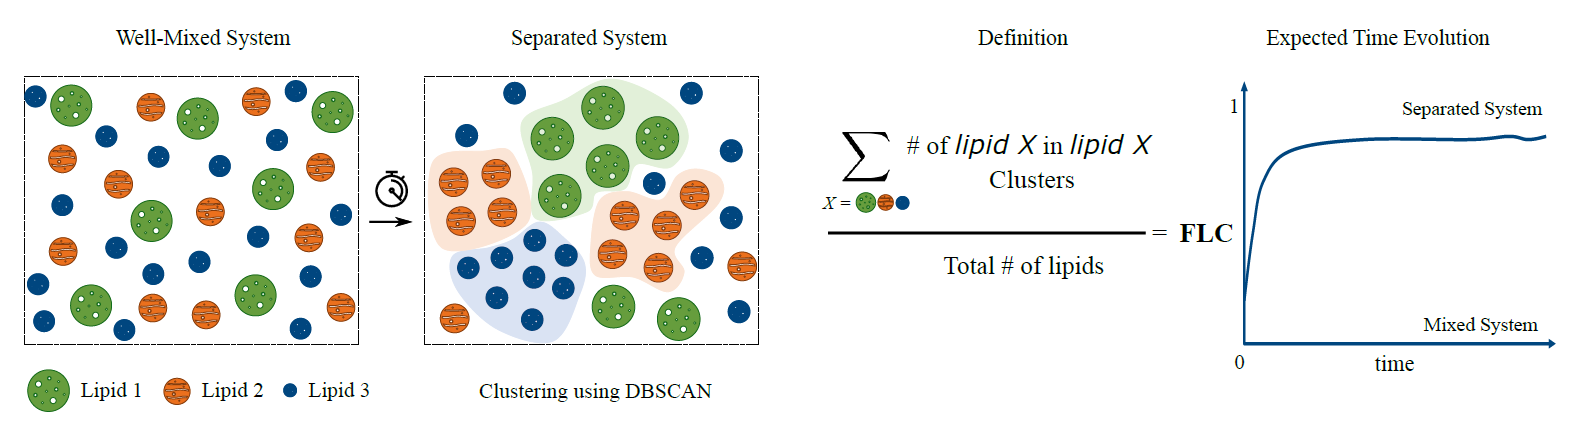
\includegraphics[width=1\linewidth]{Figures/Figure1.PNG}
\caption{a. A phase separating system evolves from a mixed state to a separated state. b. Functional form of FLC. c. FLC evolution curve for a phase separating system}
\label{fig2:view}

\end{figure}


The lipid $X_i$ cluster is defined using the Density-Based Spatial Clustering of Applications with Noise (DBSCAN) algorithm \cite{MartinEsterHans-PeterKriegelJiirgSander1996, Ester2017} as implemented in scikit-learn \cite{PedregosaF.VaroquauxG.GramfortA.MichelV.ThirionB.GriselO.BlondelM.PrettenhoferP.WeissR.andDubourgV.VanderplasJ.PassosA.CournapeauD.BrucherM.PerrotM.Duchesnay2011}.
For lipid DBSCAN clustering, instead of the default euclidean metric to calculate the distance between lipid coordinates, we used a precomputed distance matrix adjusted for periodic boundary conditions of the simulation box using LOOS.
The algorithm requires two additional input parameters: $min\_samples$ and $\varepsilon$.
We consider lipids with more than $min\_samples$ neighbors (including the lipid itself) within $\varepsilon$ radius as core lipids.
Non-core lipids still within $\varepsilon$ radius of a core lipid are considered border lipids.
A set of core lipids within $\varepsilon$ radius of each other and their border lipids forms a cluster.
All lipids that are not a part of any cluster are considered outliers.

Since lipid motion in a bilayer is constrained primarily on a plane and MARTINI beads for a lipid are of similar radii, we can use the two-dimensional version of Kepler's conjecture that the densest packing of unit disks in a plane is hexagonal close packing (Thue's Theorem).
Hence we chose 7 (6 nearest neighbors + 1 central lipid) as $min\_samples$ for all the lipid species.
However, $\varepsilon$ was chosen differently for each lipid species based on their first nearest neighbor distance from the central lipid.
We used the $xy\_rdf$ tool in LOOS to calculate an individual lipid species' first nearest neighbor distance.
From the first 8 $\mu$s MD standard simulation of each replica, we computed the radial distribution function (RDF) for a lipid species in the xy-plane. 
From the RDF plot, we found the first maxima (provided it is above 1), and the distance to the minima right after this first maximum was determined to be the first nearest neighbor distance for that lipid species.
This distance was averaged over all four replicas for a given system at a given temperature and then assigned as the respective $\varepsilon$ input.
Since nearest neighbor distance is a function of temperature, for the same lipid species in the same system, $\varepsilon$ may be different for different temperatures.
Computed $\varepsilon$, i.e., average first nearest neighbor distance for different conditions, are plotted in Supplementary Figure S1.
Additionally, we tracked auxiliary variables (AVs) that evaluate the quality of DBSCAN clustering since it is critical for defining the FLC that drives the WE equilibrium dynamics.

\subsubsection*{2. Cumulative Enrichment Index (CEI)}

We defined a density-based quantity to estimate the degree of global lipid enrichment in the system, similar to the ones that track local lipid segregation used previously \cite{Gu2019, Gu2020}.
Here, we calculated the average local density of $X_i$ lipids around a single lipid $X_{ij}$, within a cutoff radius, $\epsilon_i$, as we defined earlier for FLC estimation.
The cutoff radius, $\epsilon_i$, is also temperature dependent.
We also defined a normalization factor, $\Phi_i$, as the local density of $X_i$ lipids for a uniformly well-mixed system of similar composition.
The ratio of former respective to latter forms the enrichment index for a lipid species, $X_i$.
CEI is defined as the sum of individual enrichment index for all the lipid species in the system, as follows:

\begin{equation}
    \begin{aligned}
    \label{eq:CLT}
    \text{CEI} {}   & = \sum_{i}^{N}\Bigg[\frac{\text{Average local density of lipids $X_i$ around a single lipid $X_i$}}{\text{Local density of lipid $X_i$ for a well mixed system}}\Bigg]_{\text{$\epsilon_i(T)$}} \\
                    & =  \sum_{i}^{N} \frac{1}{\Phi_i}\frac{1}{\text{$\pi\epsilon_i^2$}}\sum_{j}\text{No. of $X_i$ lipids around $X_{ij}$ lipid in $\epsilon_i(T)$ radius}
    \end{aligned}
\end{equation}

Where $X_{ij}$ denotes $j^{th}$ lipid of $X_i$ lipid species.
The local density around $X_{ij}$ is calculated within $\epsilon_i(T)$ distance, where T is the temperature of the system.
We do correct the local density for central lipid contributions.
For the normalization factor, $\Phi_i$,  we calculated the global density of $X_i$ lipids by taking the ratio of the total number of $X_i$ lipids in the system to the $xy$-planar area of the bilayer system.
This global density is the same as the local density of $X_{i}$ lipid for a uniformly well-mixed system.
Thus CEI $>$ 3 implies that the ternary system, $N=3$, is deviating from a well-mixed state to a separated state.

\subsubsection*{3. Segregation Index (SI)}

We defined a contact-based quantity to track the homogeneity of the lipid bilayer, similar to the ones that track the mixing of beads used previously\cite{Marigo2012, Kumar2020}.
Here, we calculated the fraction of like contacts made between $X_i$ species to the total contacts made by $X_i$ as shown below:

\begin{equation}
    \begin{aligned}
    \label{eq:CLT}
    \text{SI} = \sum_{i}^{N}\Bigg[\frac{X_iX_i}{\sum_{j}^{N}X_iX_j}\Bigg]_{\text{$\epsilon_i(T)$}} = \frac{X_{11}}{X_{11} + X_{12} + X_{13}} + \frac{X_{22}}{X_{21} + X_{22} + X_{23}} + \frac{X_{33}}{X_{31} + X_{32} + X_{33}}
    \end{aligned}
\end{equation}

$X_iX_j$ denotes the contacts between lipid species $X_i$ and $X_j$ within $\epsilon_i(T)$ cutoff.
Thus for a ternary bilayer system, SI $=$ 3 implies a fully separated system, and SI $<$ 3 implies mixing.
However, for the analysis, we ignored the contribution of Cholesterol as we found that excluding the Cholesterol term did not change the functional behavior (Supplementary Info).
Hence, $\text{SI}_{\text{noCHOL}}$ effectively will have bounds [0, 2] unless otherwise stated.    

\subsection*{Weighted Ensemble Simulation}

\subsubsection*{Preparing seeding configurations for WE simulation} 
From each 8 $\mu$s replica MD simulation of a given system, the last ten frames spaced by 100 ns were collected.
Using such collected frames, we created sets of mixed and separated configurations for each system replica.
For DPPC-DAPC-CHOL and DPPC-DIPC-CHOL systems, the set of mixed configurations for a particular replica came from the respective 423 K and 450 K simulation frames. 
The set of separated configurations for a replica comes from the respective 298K and 323K simulation frames.
For the DPPC-POPC-CHOL system, sets of mixed and separated configurations for a replica came from the 450 K and 298K simulation frames, respectively.
To enhance the convergence of WE equilibrium simulations, we decided to seed each simulation from mixed and separated states and let the enhanced sampling cover the transition between them.

\subsubsection*{Running WE simulations} 
We ran weighted Ensemble equilibrium simulations using the WESTPA 1.0 software package\cite{Zwier2015} closely following the previously established protocol\cite{Bogetti2019}.
The collective variable was divided into 30 dynamic bins using the minimal adaptive binning scheme (MAB)\cite{Torrillo2021}.
For each replica, a target number of 4 short simulations, or "walkers" per bin, were started in parallel from the mixed and the separated configurations prepared earlier.
After every resampling interval of 1 ns, the collective variable was evaluated to initiate the merging and splitting of walkers to maintain the target number of walkers per bin.
A short one ns MD run of all the walkers and subsequent resampling, according to the standard WE algorithm, constituted 1 WE iteration. 
We conducted 500 WE iterations for each replica.
We used GROMACS 2020.3 engine to propagate with the same parameters used for standard MD simulations described earlier.
A WE Equilibrium Dynamics (WEED) reweighting protocol\cite{Bhatt2010, Suarez2014}, implemented in WESTPA 1.0, was used to accelerate the convergence of WE walkers into an equilibrium.
The reweighting is done every 10 WE iterations.
Four WE replicas were simulated at multiple temperatures for the DPPC-DAPC-CHOL, DPPC-DIPC-CHOL, and DPPC-POPC-CHOL lipid bilayer systems. 
All WE simulations ran using the Intel Xeon E5-2695 and Tesla K20Xm GPUs in the BlueHive supercomputing cluster of the Center for Integrated Research and Computing at the University of Rochester.   

\subsubsection*{Analysis of WE simulations}
The probability distribution of CV and AVs for each replica, as a function of WE iterations, was constructed using $w\_pdist$ and $plothist$ tools in WESTPA.
Using this distribution, we monitored the evolution of each WE replica simulation and the convergence.
We used the $w\_mult\_west$ tool in WESTPA to combine data from four WE replicas of a system at a given temperature.
We then constructed the respective Free Energy Surface (FES) from the combined probability distribution of a system.
To check populations in different states and the flux between states  $w\_ipa$ tool was used.

\section*{Results}

Consistent with previous studies from which they are adapted, the standard CG MD simulations of DPPC-(DA/DI)PC-CHOL systems phase separates into $\text{L}_{\text{o}}$ and $\text{L}_{\text{d}}$ regions.
$\text{L}_{\text{o}}$ region enriched in saturated lipid, DPPC, and Cholesterol. 
$\text{L}_{\text{d}}$ region is enriched with unsaturated lipids (DA/DI)PC.
The DPPC-POPC-CHOL system showed low to no separation.
This section compares how different variables track phase separation propensity in lipid bilayers using standard CG MD simulations.
We then compare the convergence of WE simulation to the choice of collective variable.
Finally, we present the free energy landscapes of lipid bilayer systems obtained using WE simulations and discuss reusing the data generated to form other intuitions and applications.

\subsection*{Tracking phase separating lipid bilayers}

To evaluate how collective variables, FLC, and other auxiliary variables track phase separation in lipid bilayers,
from standard CG MD, we traced the time evolution of each variable for different systems at different temperatures.
Figure 3 illustrates the temporal evolution of FLC, CEI, and $\text{SI}_{\text{noCHOL}}$ for DPPC-(DA/DI/PO)PC-CHOL systems at 298K, 323K, 423K, and 450K.
For DPPC-(DA/DI)PC-CHOL systems, the variables capture a single transition between a mixed state and a separated state.
Also, the systems reside dominantly in a separate state after the transition in the standard CG simulation.
Interestingly, for relatively slow separating DPPC-DIPC-CHOL, CEI and $\text{SI}_{\text{noCHOL}}$ tracks a relatively slower state transition than FLC.
However, for the DPPC-POPC-CHOL system, the variables capture a single state corresponding to a mixed system and no transition.
Nevertheless, it is worth noting that FLC, CEI, and $\text{SI}_{\text{noCHOL}}$ capture the effect of temperature in all systems, including the negative control that does not phase separate.
These variables even capture the subtle differences in phase-separating propensity between systems.
For example, at 298K, the plateaued region of the FLC, CEI, and $\text{SI}_{\text{noCHOL}}$ curves are higher for the DPPC-DAPC-CHOL system than the DPPC-DIPC-CHOL system.
This is expected as (a) the lipid chain mismatch between saturated and unsaturated lipid species and (b) the number of double bonds in unsaturated lipid species is more in the DPPC-DAPC-CHOL than DPPC-DIPC-CHOL system.
Both these factors have previously been shown to influence lipid phase separation kinetics and domain stability\cite {Fowler2016, Lin2016}.
Thus we have a set of low-dimensional variables that can (a) represent the global dynamics of the lipid bilayer system,
(b) distinguish and track the transition between mixed and separated states, (c) capture the temperature effects,
and (d) based on the composition of the system.
The time evolution of other auxiliary variables can be found in Fig SX.
\\

\subsection*{Choice of collective variables for WE simulations}

Since the density based, CEI, contact-based $\text{SI}_{\text{noCHOL}}$ and clustering based FLC tracks bilayer lipid separation similarly,
we decided to use them as progress coordinates to drive the WE simulation.
However, the free energy landscapes generated using these variables, after running 500 WE iterations, give conflicting results for the same system.
As shown in Figure 4A, for the test system DPPC-DIPC-CHOL replica at 323K, the free energy landscape do not agree with each other despite the number of WE iterations used to construct them being identical.
From CEI free energy landscape, we see both states are equally likely.
$\text{SI}_{\text{noCHOL}}$ landscape suggests a mixed state is more likely than a separated state.
However, both these results deviate from what we observe with standard CG MD simulation,
where the DPPC-DIPC-CHOL system slowly separates into $\text{L}_{\text{d}}$ and $\text{L}_{\text{o}}$ regions and stay separated for the most of simulation.
Moreover, disagreement of free energy curves as a function of WE iteration blocks used to generate them suggests that the underlying sampling needs to converge more.
On the other hand, FLC free energy landscape shows that the separated state is favorable, but the free energy barrier between the two states is small.
Additionally, there is a convergence between FLC free energy curves as we proceed with WE iterations.
Thus, all three free energy landscapes show a double well, identifying two states but disagreeing on the state the system is most likely to be in and the relative free energy difference between states.
Interestingly, if we monitor the evolution of configurational distributions of each variable as a function of WE iterations, all three show a converged behavior, as shown in Fig 4B.

These conflicting results raise the following questions: Why do variables that make perfect sense while tracking the system in standard CG MD simulation gives a different free energy landscape after WE simulation?
Why do CEI and $\text{SI}_{\text{noCHOL}}$ that show converged configurational distributions as a function of WE iterations, does not give converged free energy curves with each other as WE proceed?

The configurational distribution of collective variables staying mostly undisturbed in two states (Fig 4B) and
the free energy curves struggling to converge on the state basins and free energy barrier for CEI and $\text{SI}_{\text{noCHOL}}$ landscapes (Fig 4C) 
suggest that there might not be adequate state crossing of walkers populating each state.
Hence we decided to check the flow rate of probability across the states.
To calculate the flux between states, we need to define the states for each collective variable.
We define mixed and separated states as CEI = [0.0, 3.9] and [4.4, 6.0], $\text{SI}_{\text{noCHOL}}$ = [0.0, 1.3] and [1.4, 2.0], and FLC = [0.0, 0.575] and [0.65, 1.0] respectively.
Please note that the state bounds are chosen based on visual inspection of the corresponding free energy landscapes in Fig 4A.
The choice is arbitrary but ad hoc enough to give us a picture of what is happening. 
Fig 4C shows the mean flux from mixed to separated state and vice versa in WE simulation driven using each collective variable.
Here, mean flux is calculated for a window of 10 WE iterations as the WEED reweighting protocol is done every ten iterations to accelerate the convergence.
The peaks in these plots imply probability crossing states.
For CEI, no state crossing occurs between mixed to demixed, and vice versa during WE simulation.
For $\text{SI}_{\text{noCHOL}}$, the state crossing back and forth is practically zero during the first few hundreds of WE iterations.
Meanwhile, for FLC, flux into and out of the states is relatively higher and more immediate than the other two variables.
These results are supported by the corresponding state population evolution as a function of WE iterations, as shown in Fig 4D.
Here, the normalized walker population occupying a specific state is calculated for 10 WE iterations, similar to Fig 4C.

The walkers crossing bins and thereby constituting a flow of probability between states is crucial for the success of a WE equilibrium simulation\cite{Zuckerman2017}.
Thus these results suggest that for CEI and $\text{SI}_{\text{noCHOL}}$ variables, the initial distribution of walkers is not disturbed throughout the WE simulation.
Without sufficient state crossing, the initial configurational distribution is not relaxing into a well-sampled equilibrium distribution for WE simulations driven by CEI and $\text{SI}_{\text{noCHOL}}$ even after 500 iterations. 
This explains why in free energy landscapes associated with CEI and $\text{SI}_{\text{noCHOL}}$, we do not see converged free energy curves as WE proceed.
However, as WE proceed, we see good state crossing and relatively well-converged free energy curves for FLC. 
The combined results from standard CG MD and WE simulations suggest that CEI and $\text{SI}_{\text{noCHOL}}$ are suitable proxy labels for phase separation. However, a poor choice for a collective variable to drive WE simulations.
We also found that free energy curves generated by FLC-driven WE simulation are consistent across replicates (Fig SX).
Hence we decided to go forward with FLC-based WE simulation to enhance the sampling of phase separation events in lipid bilayer systems to understand the underlying thermodynamics.
\\ 
\subsection*{Free energy landscapes of lipid bilayer systems}

Figure 5 shows the free energy profiles of DPPC-DAPC-CHOL, DPPC-DIPC-CHOL, and DPPC-POPC-CHOL lipid bilayer systems.
Each curve is generated by averaging four WE replica simulations, as mentioned in the Methods section.
Individual replica contribution is obtained by averaging the last ten iterations of the respective replica WE simulation (491-500). 
The positive control, DPPC-DAPC-CHOL system that readily phase-separates, has a double well behavior at 323K and 353K.
However, both basins correspond to relatively high FLC.
In addition to the free energy curve at 423 K, we see that regardless of high temperature, this system prefers to be in configurations where more than 60\% of lipids are in some clusters.
For the negative control, DPPC-POPC-CHOL system, the free energy curves at 298K and 423K have single basin nature and correspond to a low fraction of lipids preferring to be in any clusters.
For the test system, DPPC-DIPC-CHOL system, as the temperature increases, the characteristic double-well transition to single-well curves, and the width of free energy curves decreases.
In general, FLC-based free energy landscapes capture the role of lipid species constituting the bilayer system in its phase separation.
Moreover, the effect of temperature in decreasing the propensity of a lipid bilayer to separate is evident in all systems.
Please note that though the expectation of clustering-based FLC is to track the formation of domains in a lipid bilayer, the fact that it also neatly captures the temperature effect, even for the negative control, suggests the robustness of FLC as the collective variable.
%\subsection*{Reusing simulation data}

\subsection*{Reconstructing free energy landscapes}
One outcome of WE simulation is the curated ensemble of diverse trajectories/walkers.
By construction, WE resampling ensures that the weights associated with these walkers are unbiased.
Thus, we can reuse these weights to examine other variables of choice post-simulation.
Assuming the initial configurational distribution relaxed into an equilibrium distribution during WE simulation driven by FLC (see Discussion), 
by reusing the weights, we have reconstructed analogous free energy landscapes with collective variable candidates that underperformed.
Fig 6 A and B show reconstructed free energy landscapes with CEI and $\text{SI}_{\text{noCHOL}}$ by combining the weights from the last ten iterations of four replicas for each system.

\textbf{$\bigotimes$ I need to construct free energy landscapes similar to Fig 4 A where I plot free energy curves w.r.t WE iteration for CEI and SI using FLC driven WE simulation data. And show that unlike Fig 4 A, now the curves converge. Working on that!! $\bigotimes$}

The WESTPA framework allows one can resume the WE simulation using variables of choice using the weights from existing ensemble\cite{Zhang2010, Zwier2015}.
Hence by reusing the unbiased weights on the trajectory ensemble we obtained from a reasonably converged WE simulation,
we can rescue the underperformance of WE simulation due to the initial choice of poor collective variable.

\subsection*{$\Delta\Delta$G profile of lipid system}

From free energy landscapes of lipid bilayer at various temperatures, we can create a $\Delta\Delta$G profile by defining an FLC cutoff between mixed and separated states.
As seen in Fig 5 A, the concept of state basins is different for a system at different temperatures.
In high temperatures, the notion of two states - mixed and separated - breaks down as the double-well behavior of free energy curves turns into a single well. 
One trivial solution would be to define a rigid FLC cutoff for a system.
However, a caveat for this approach, as seen in Fig 5 A, is that the free energy basin for a specific state of the DPPC-DIPC-CHOL system is different for the respective state basin for the DPPC-DAPC-CHOL system.
So a rigorous FLC cutoff for the state definition of a system may need to be clarified in another phase-separating system.
Thus, to showcase the capability of the pipeline we have presented here, we define an ad hoc cutoff, FLC = 0.5, for a general lipid system.   
i.e., we make an arbitrary choice of a separated lipid bilayer if more than 50\% of lipids in the system is part of some clusters.
Figure 7 shows the $\Delta\Delta$G curve for the DPPC-DAPC-CHOL system as a function of temperature for FLC=0.5 cutoff.
Even though we can see that $\Delta\Delta$G curve for mixed to separated transition is crossing $\Delta\Delta$G=0 line, indicating the corresponding melting temperature,
we advise the reader to exercise caution while interpreting this result as we have a coarse-grained model, an arbitrary cutoff, and lack of experimental data to compare it with for given composition.
However, we want to highlight the capability of this proof-of-concept pipeline we created to achieve $\Delta\Delta$G profiling for a phase-separating system.
We expect more accurate profiling by using a more accurate all-atom model for our system with more rigorous methods for defining phase separation in FLC space that account for 
varying propensity as a function of temperature and system composition.
Fig SX shows the sensitivity of FLC cutoffs on $\Delta\Delta$G profile for a given system.

\section*{Discussion}

Here we propose a proof-of-concept pipeline to construct \textbf{F}re eenergy \textbf{L}andscape \textbf{O}f \textbf{P}hase \textbf{S}eparating \textbf{S}ystems (\textbf{FLOPSS}) by realizing multiple transition events using WE strategy.
Even though our systems of interest are lipid bilayers, using appropriate model resolution and collective variables can generalize this pipeline to any system that phase separates.
The modular pipeline is outlined in Figure 8, with different sublayers that constitute each module.
Given the limitation of the coarse-grained model, free energy landscapes generated by FLOPSS in our positive, test, and negative lipid bilayer system qualitatively agrees with previous literature.
For a more quantitative comparison, the next logical step is to use all-atom lipid models.
Thus we can investigate both the thermodynamics and kinetics of phase-separating lipid bilayers.
Interestingly, many more tools are available from the WE community as the WE strategy has been used predominantly for determining the kinetics of the different systems.

In this work, we have proposed a simple yet efficient collective variable that simultaneously tracks phase separation and drives WE simulation, ensuring sufficient state crossing with reasonable convergence of configurational distribution. 
We give yet another example of why collective variable choice is crucial for the success of enhanced sampling protocols. 
The flux analysis presented here only answers how much some proxy labels drive WE simulation better than others.
However, our work still needs to explain why that is the case.
Thus, a more thorough and systematic analysis of the sensitivity of WE simulation on the choice of collective variable is needed and is unfortunately beyond the scope of this work.

We also acknowledge that certain parameter choices for FLOPSS need further optimization.
For example, the current choice of 1 ns as resampling interval, $\tau$, for WE simulation is arbitrary.
Thus a systematic study of $\tau$ is needed.
Similarly, we have chosen an arbitrary 10-iteration window between successive WEED reweighting to accelerate the convergence.  
There is room for optimization here as well.
Evidence of finite simulation box size effect on domain formations in phase separating lipid bilayer has been reported previously\cite{Pantelopulos2017}.
Thus we need to investigate any critical size dependence of free energy landscapes generated by FLOPSS.
We acknowledge that the current crude pipeline has scope for further optimization. 

In summary, we have developed and validated a new framework that can directly compute the thermodynamics associated with phase separation from simulation.
We have also demonstrated the potential reuse of a reasonably converged WE equilibrium simulation driven by a good collective variable to explore other variables which otherwise constitute a poor choice for driving WE simulation.
Thus, we can increase the effectiveness of WE simulation without compromising on computational cost.
Moreover, we also showcase the potential of FLOPSS to construct a $\Delta\Delta$G profile of the system under study to investigate the melting properties.

The FLOPSS pipeline proposed here can be applied to study (a) perturbations in the free energy landscape of lipid bilayer as new species are introduced, such as other lipids, peptides, small molecules, etc.
(b) the effects of symmetric and asymmetric bilayer leaflets in phase separation thermodynamics,
(c) the differences in free energy landscapes made from CG and all-atom models 
(d) to derive bilayer properties from an enhanced sampled configurational space than standard MD simulation, etc. 
Deviating from the lipid bilayer system, we also wish to make FLOPSS more rigorous by testing FLOPSS on toy systems that have simple analytical solutions to compare with. 
We want to highlight that by generalizing the collective variable FLC to track clustering in 3D space, FLOPSS can also be extended to other instances of biological phase separation.
However, this assumes that a reasonable model, forcefield, and computational resources are available to tackle such complex phase-separating systems via MD simulations.




% ------------------------- %
% Uncomment if using bibtex (default)
\bibliography{PhaseSeparationArticle}

\section*{Supplementary Material}

\subsection*{Auxiliary Variables}

For each lipid species, $X$ in the system, we calculated the following, 

1. Number of $X$ clusters in the system under study.

2. Fraction of $X_i$ lipids in $X$ clusters

3. Fraction of $X_i$ lipids in $X$ core lipids.

4. Mean Silhouette Coefficient (MSC) of $X_i$ Clusters, as implemented in scikit-learn.

Silhouette Coefficient is a method used to evaluate the clustering done by any technique, especially if ground truth labels are unknown. 
Here, for a $X_i$ lipid in the cluster, mean intra-cluster distance (a) from other $X_i$ lipids in the cluster is found.  
Similarly, for a $X_i$ lipid in the cluster, the mean nearest-cluster distance (b) is also calculated.
While the former assesses the 'cohesion' of a given $X_i$ lipids with other $X_1$ lipids in a cluster, the latter assesses the 'separation' from the nearest cluster.
Thus, Silhouette Coefficient for a $X_i$ lipid, s, is defined as below,

\begin{equation}
\label{eq:SC}
\text{s} = \frac{b - a}{max(a,b)}
\end{equation}

The Mean Silhouette Coefficient of $X_i$ Clusters is given by the mean $s$ over all non-outlier $X_i$ lipids.
Here, we have omitted the MSC calculations for cases when there are no clusters or just one cluster detected by DBSCAN. 
MSC is bound between and -1 and 1.
A high positive value corresponds to well segregated dense clusters, while a low negative value implies that lipids are assigned to clusters incorrectly.  

\end{document}